% !TeX program = pdflatex

\documentclass[11pt,a4paper]{article}
\usepackage{graphicx}
\graphicspath{{./}{../../}{../../figures/}}

\usepackage[margin=1in]{geometry}
\usepackage[T1]{fontenc}
\usepackage[utf8]{inputenc}
\usepackage[american]{babel}
\usepackage{lmodern}
\usepackage{microtype}
\usepackage{authblk}
\usepackage[dvipsnames]{xcolor}
\usepackage[textsize=small]{todonotes}
\usepackage{amsmath,amssymb,mathtools}
\usepackage{booktabs,threeparttable,tabularx,array}
\newcolumntype{L}[1]{>{\raggedright\arraybackslash}p{#1}}
\usepackage{caption}
\usepackage{float}
\usepackage{placeins}

\usepackage[most]{tcolorbox}

\newtcolorbox{plainlanguagebox}{
  breakable,
  colback=DemBlue!6,
  colframe=DemBlue!70!black,
  coltitle=white,
  fonttitle=\bfseries,
  title={In simple terms},
  boxrule=0.8pt,
  arc=2mm,
  left=8pt,
  right=8pt,
  top=7pt,
  bottom=7pt
}

\newtcolorbox{resultsbox}{
  colback=RecoveryGreen!6,
  colframe=RecoveryGreen!70!black,
  coltitle=white,
  fonttitle=\bfseries,
  title={How to interpret the results},
  boxrule=0.8pt,
  arc=2mm,
  left=8pt,
  right=8pt,
  top=7pt,
  bottom=7pt
}

\newtcolorbox{payoffbox}{
  colback=DemBlue!4,
  colframe=DemBlue!70!black,
  coltitle=white,
  fonttitle=\bfseries,
  title={A simple payoff comparison},
  boxrule=0.8pt,
  arc=2mm,
  left=8pt,
  right=8pt,
  top=7pt,
  bottom=7pt
}

\newtcolorbox{keyinsightbox}{
  colback=ExecOrange!7,
  colframe=ExecOrange!80!black,
  coltitle=white,
  fonttitle=\bfseries,
  title={Central insight},
  boxrule=1pt,
  arc=2mm,
  left=8pt,
  right=8pt,
  top=7pt,
  bottom=7pt
}

\usepackage{tikz}
\usetikzlibrary{positioning,arrows.meta,fit,calc}
\usepackage{csquotes}
\usepackage[hidelinks]{hyperref}
\usepackage[capitalize,noabbrev]{cleveref}
\usepackage[
  backend=biber,
  style=authoryear,
  dashed=false,
  doi=false,
  isbn=false,
  url=false,
  arxiv=false,
  uniquename=false,
  uniquelist=false
]{biblatex}
\addbibresource{../../references.bib}
\renewcommand*{\bibfont}{\small}

\definecolor{DemBlue}{HTML}{264653}
\definecolor{ExecOrange}{HTML}{E76F51}
\definecolor{RecoveryGreen}{HTML}{2A9D8F}
\definecolor{LightBlue}{HTML}{EAF2F4}
\definecolor{LightOrange}{HTML}{FBEDE9}
\definecolor{PersistPurple}{HTML}{6D597A}
\newcommand{\Dproc}{\textsf{D}}
\newcommand{\Aproc}{\textsf{A}}
\newcommand{\ind}[1]{\mathbb{1}\{#1\}}

\title{
\includegraphics[width=0.32\textwidth]{utu_logo.pdf}\\[1.2em]
\textbf{\input{../../title.txt}\unskip}\\[0.35em]\large Research Plan for Ethical Review}
\author[1,2]{\textsc{Hector Bahamonde}}
\affil[1]{INVEST Research Flagship Centre, University of Turku, Finland}
\affil[2]{Social Science Research Institute, \AA bo Akademi University, Finland}
\date{\textbf{Principal Investigator and project contact:} Janne Tukiainen, Professor, Turku School of Economics, University of Turku; \href{mailto:janne.tukiainen@utu.fi}{janne.tukiainen@utu.fi}\\[0.4em]Version 2.0 --- 31 August 2026}
\IfFileExists{upquote.sty}{\usepackage{upquote}}{}
\begin{document}
\pagenumbering{gobble}
\maketitle

\begin{abstract}
Democratic backsliding often proceeds through lawful democratic choices that weaken citizens' control over what happens next. This project asks whether citizens vote to restore an approval right they supported surrendering once its crisis-based justification recedes. In a one-session public-goods experiment with 300 participants in Finland, five-person groups decide whether an unknown leader's proposal requires citizen approval or takes effect directly. Acting without approval initially combines a higher fund rate with assured implementation of the leader's equal allocation. Structural recovery improves public-service conditions and raises the approval-constrained rate to match direct implementation, while the leader's powers and decision rules remain unchanged. Comparing randomly assigned recovery and persistence pools identifies whether recovery causes previous supporters of direct implementation to vote for group approval. The experiment captures a demand-side microfoundation of executive aggrandizement: citizens can use one democratic decision to weaken a later constraint and another to vote to take that control back.
\end{abstract}

\vspace{2cm}

\begin{center}
\small\textbf{Experiment prototype (production phase):} \\ \url{https://panel-lab-experiment.onrender.com}
\end{center}

\clearpage
\pagenumbering{arabic}
\setcounter{page}{1}

\section{Research Question and Contribution}

Democratic backsliding depends not only on leaders who weaken constraints but also on citizens who authorize them. This project studies a narrow demand-side microfoundation of executive aggrandizement: the citizen-level authorization through which a lawful democratic decision weakens a constraint on one-person authority. It asks: \emph{after a crisis recedes, do citizens who supported decisions without their approval vote to restore that right?} This within-person change in institutional support is the {\bf (\emph{un})democratic reversal} the project seeks to explain.

We build on the democratic backsliding and public-good games literatures. Contemporary backsliding often advances without ending elections: citizens may support elected officials or lawful rule changes that reduce the approval, oversight, or veto constraints governing later decisions \parencite{Bermeo2016}. The politically relevant step is therefore not necessarily an explicit vote against democracy, but a \emph{democratic} vote that makes subsequent authority \emph{less} constrained. Threat and policy benefits can make citizens more tolerant of such constraints being weakened \parencites{HetheringtonSuhay2011}{Goodman2021}{0b3bf}, while laboratory evidence shows that gridlock can increase support for executive special powers \parencite{FortezaMussioPereyra2024}.

This literature mainly explains movement toward less constrained authority. Our contribution is to follow the reverse movement: once the crisis-based benefit recedes, do the same citizens vote to restore the approval right they previously supported surrendering? Observing that second choice turns reversal into a consequential decision over an institutional constraint rather than a stated evaluation of democracy.

Public-good games supply the economic reason for weakening approval. Voluntary provision is vulnerable to free riding---keeping one's points while others fund the shared service---and declining cooperation, whereas centralized enforcement can coordinate contributions \parencites{FehrGachter2000,FischbacherGachter2010,Hamman2011}. Experiments also show that voting over institutions changes their performance \parencites{DalBo2010,SutterHaignerKocher2010,MarkussenPuttermanTyran2014}. Our experimental design joins these literatures by making citizen approval both institutionally meaningful and economically costly.

In each round, five citizens begin with 20 points each and vote between two rules for managing a shared public-services fund. Under both rules, the software selects a leader only after the vote, choosing among those who have served least often and breaking ties randomly. The leader proposes how many points every citizen places in the fund and whether any collected points move to the leader's payoff. Fund points are multiplied and the resulting group return is divided equally.

Under the approval-constrained rule (\Dproc), at least three of the other four citizens must approve the complete proposal. Rejection returns the group to voluntary individual allocations. Under automatic implementation (\Aproc), the same proposal takes effect without that approval vote. A matching pool contains 10 or 15 citizens and is reshuffled into two or three temporary groups of five before each round. Thus, the democratic ballot selects an approval rule, not a known leader or proposal.

Everyone begins with a public-service crisis: \enquote{\emph{Parliament has failed to pass a budget for eight months, healthcare waiting times have doubled, and planning for public services has stalled.}} During Block 1, each fund point creates 1.50 group points under \Dproc{} and 2.50 under \Aproc{}. Direct implementation therefore has a one-point productivity premium and guarantees that the leader's proposal is implemented. Afterward, each matching pool receives {\bf institutional recovery} or {\bf institutional persistence}. Recovery is one structural package: public-service conditions improve and the \Dproc{} rate rises to 2.50. Persistence retains the crisis and the 1.50 rate. The \Aproc{} rate and decision rule remain fixed.

The payoffs make the choice consequential; {\bf the \emph{allocation of decision rights} connects it to democratic backsliding}. A citizen who votes for \Aproc{} supports surrendering an approval vote before knowing the leader or proposal. A later vote for \Dproc{} supports restoring that safeguard after the crisis-based productivity advantage disappears. \emph{The experiment therefore observes whether citizens vote to take back a specific constraint on authority, rather than inferring reversal from a survey declaration}.

\begin{plainlanguagebox}
Five citizens vote before seeing who will lead or what the leader will propose. Under \Dproc{}, three of the other four citizens must approve the proposal; rejection returns everyone to individual fund allocations. Under \Aproc{}, the proposal takes effect directly. In Block 1, these methods use rates of 1.50 and 2.50, respectively.

After Block 1, recovery improves public-service conditions and raises \Dproc{} to 2.50; persistence leaves the crisis and rate gap in place. Among previous \Aproc{} supporters, a later \Dproc{} vote supports restoring the approval right. Comparing recovery with persistence identifies how much the structural recovery package changes that reversal.
\end{plainlanguagebox}

\begin{keyinsightbox}
A decision can be democratically authorized while weakening the democratic constraints that govern what happens next. This resembles contemporary backsliding, which often proceeds through elections and formally lawful institutional changes rather than an outright abolition of democracy \parencite{Bermeo2016}.

In the experiment, the first majority vote is democratic. A citizen who chooses \Aproc{} votes to let an unknown leader's later allocation and transfer take effect without the other citizens' approval. That vote removes a specific constraint while leaving the institutional ballot itself intact. A later vote for \Dproc{} supports restoring the approval right the citizen previously voted to surrender.

\medskip
\textbf{What matters is that citizens use one democratic decision to weaken their control over subsequent decisions---and can later vote to take that control back.}
\end{keyinsightbox}


\section{Theory}

\subsection{Crisis and the productivity premium}

A crisis can make action without approval attractive when ordinary procedures produce delay or failed coordination. The experiment gives this argument material consequences. In Block 1, proposals requiring approval (\Dproc) use a 1.50 fund rate, while proposals implemented directly (\Aproc) use 2.50. Under \Dproc{}, rejection also returns the group to voluntary contributions and possible free riding. Direct implementation therefore offers both a productivity premium and assured implementation of the leader's equal allocation \parencites{FehrGachter2000,FischbacherGachter2010,Hamman2011}.

The personal-transfer option makes the institutional constraint consequential. The leader may propose moving up to 20 fund points to their own payoff under either procedure. Under \Dproc{}, the other citizens see that transfer before implementation and can reject it; under \Aproc{}, they observe it only after it has taken effect. The experiment therefore concerns approval over discretion, not the prevalence of corruption in Finland.

\paragraph{H1: Authorization under crisis.} During Block 1, citizens will increasingly support direct implementation (\Aproc{}) when its productivity and coordination advantages produce better outcomes; larger observed transfers will reduce subsequent support.

\subsection{Citizen authorization and democratic constraint}

The institutional ballot occurs before leader selection and before the proposal. A vote for \Aproc{} therefore authorizes a rule, not a known person or action: the citizen relinquishes participation in approving the next binding decision. A vote for \Dproc{} retains that approval right. {\bf Thus, our design provides an abstract microfoundation of \emph{executive aggrandizement}, in which a \emph{democratic} choice \emph{weakens} the constraint governing what follows} \parencites{Bermeo2016,FortezaMussioPereyra2024}.

\paragraph{H2: Approval and discretion.} Approval will decline as proposed personal transfers increase. Anticipating rejection, leaders operating under \Dproc{} will propose smaller transfers than leaders whose proposals take effect directly. Because groups choose the institutional rule themselves, these patterns describe behavior within the chosen rules rather than a separate randomized effect.

\subsection{Recovery and democratic reversal}

Recovery is assigned at the matching-pool level. Pool \(g\) contains 10 or 15 participants, who are reshuffled into two or three temporary groups of five before each round; within each group, three votes produce a majority. The entire pool receives the same Block-2 condition: \(T_g=1\) denotes recovery and \(T_g=0\) persistence. Let \(m_{gb}\) denote the approval-constrained fund multiplier in pool \(g\) and block \(b\). The productivity premium for direct implementation is

\begin{equation}
\delta_{gb}=2.50-m_{gb}
\label{eq:productivity-premium}
\end{equation}

Everyone faces \(\delta_{g1}=2.50-1.50=1\) in Block 1. Recovery is deliberately implemented as one structural package: participants learn that public-service conditions improved and \(m_{g2}\) rises to 2.50, setting \(\delta_{g2}=0\). Persistence reports that the crisis continues and keeps \(m_{g2}=1.50\), so \(\delta_{g2}=1\). The leader-selection rule, proposal set, approval threshold, rejection-to-voluntary-allocation rule, and \Aproc{} rate remain fixed.

The recovery--persistence comparison identifies the total causal effect of structural recovery on (un)democratic reversal. Among final-round Block-1 supporters of \Aproc{}, the analysis compares later \Dproc{} votes in recovery pools (\(T_g=1,\delta_{g2}=0\)) with those in persistence pools (\(T_g=0,\delta_{g2}=1\)). The public-service description and production rate jointly define recovery: the text states what changed, while the rate makes that change materially consequential inside the game. The estimand therefore concerns their combined effect rather than separate framing and payoff effects. Persistence supplies the counterfactual in which both the crisis and premium remain.



\paragraph{H3: Immediate restoration.} Among participants who vote for \Aproc{} in Block 1's final round, recovery will increase the probability of voting for \Dproc{} in Block 2's first round.

\paragraph{H4: Sustained reversal.} Among the same participants, recovery will increase the probability of voting for \Dproc{} in Block 2's final round.

\section{Experimental Design}

\subsection{Overview}

Each laboratory cohort completes one session lasting approximately 60 minutes, with two ten-round blocks. Subject to ethical review in September 2026, data collection at the PCRC Decision Laboratory is planned for 1--31 October 2026. Participants remain in matching pools of 10 or 15 and are reshuffled into anonymous five-person groups before every paid round. After Block 1, each entire pool is assigned to recovery or persistence, learns whether public-service conditions improved or remained strained, and sees its Block-2 fund rates. Participants therefore interact repeatedly without forming stable five-person teams. In the figures, \(p_i\) identifies participant \(i\).

\begin{figure}[H]
\centering
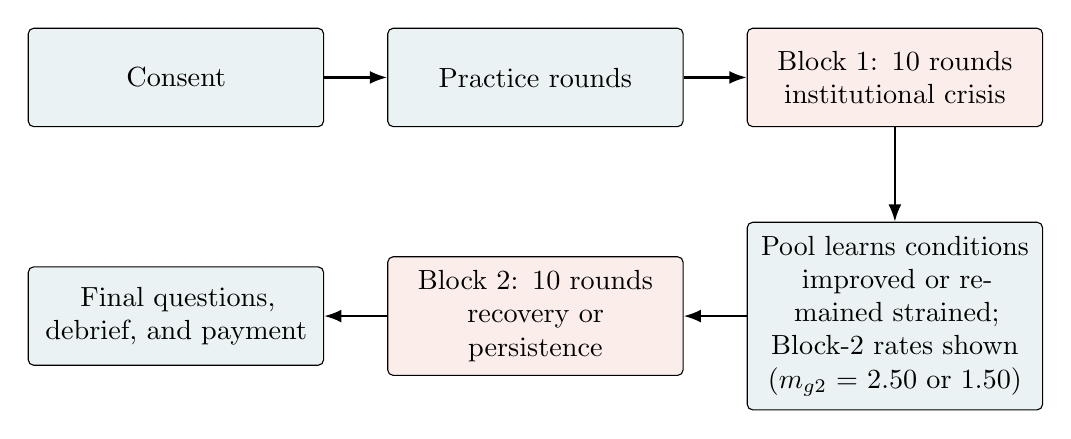
\begin{tikzpicture}[
  node distance=8mm and 8mm,
  box/.style={draw,rounded corners=2pt,align=center,text width=3.4cm,minimum height=1.25cm,inner sep=5pt},
  arr/.style={-{Latex[length=2.2mm]},thick}
]
\node[box,fill=LightBlue] (base) {Consent};
\node[box,fill=LightBlue,right=of base] (practice) {Practice rounds};
\node[box,fill=LightOrange,right=of practice] (blockone) {Block 1: 10 rounds\\institutional crisis};
\node[box,fill=LightBlue,below=12mm of blockone] (random) {Pool learns conditions\\improved or remained strained;\\Block-2 rates shown\\($m_{g2}=2.50$ or $1.50$)};
\node[box,fill=LightOrange,left=of random] (blocktwo) {Block 2: 10 rounds\\recovery or persistence};
\node[box,fill=LightBlue,left=of blocktwo] (finish) {Final questions,\\debrief, and payment};
\draw[arr] (base) -- (practice);
\draw[arr] (practice) -- (blockone);
\draw[arr] (blockone) -- (random);
\draw[arr] (random) -- (blocktwo);
\draw[arr] (blocktwo) -- (finish);
\end{tikzpicture}
\caption{One-session sequence. Each paid round includes an institutional ballot, leader proposal, implementation, feedback, and rematching.}
\label{fig:design}
\end{figure}

\begin{figure}[H]
\centering
\resizebox{0.94\linewidth}{!}{%
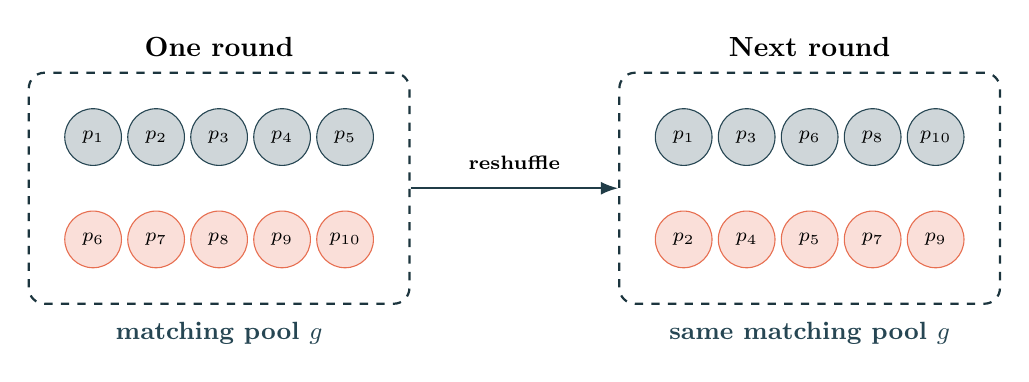
\begin{tikzpicture}[
  font=\small,
  >=Latex,
  person/.style={circle,draw,minimum size=7.2mm,inner sep=0pt,font=\scriptsize\bfseries},
  groupone/.style={person,draw=DemBlue,fill=DemBlue!22},
  grouptwo/.style={person,draw=ExecOrange,fill=ExecOrange!22},
  poolbox/.style={draw=DemBlue!75!black,dashed,rounded corners=2mm,line width=0.8pt,inner sep=4.5mm},
  flow/.style={-{Latex[length=2.2mm]},line width=0.8pt,draw=DemBlue!85!black}
]

% One paid round
\node[font=\bfseries] at (2.65,3.70) {One round};
\foreach \lab [count=\k from 0] in {1,2,3,4,5} {
  \node[groupone] (firsta\lab) at ({1.05+0.80*\k},2.55) {$p_{\lab}$};
}
\foreach \lab [count=\k from 0] in {6,7,8,9,10} {
  \node[grouptwo] (firstb\lab) at ({1.05+0.80*\k},1.25) {$p_{\lab}$};
}
\node[poolbox,fit=(firsta1)(firsta5)(firstb6)(firstb10)] (firstpool) {};
\node[font=\small\bfseries,text=DemBlue,anchor=north]
  at ($(firstpool.south)+(0,-0.10)$) {matching pool $g$};

% Next paid round: same pool, new groups
\node[font=\bfseries] at (10.15,3.70) {Next round};
\foreach \lab [count=\k from 0] in {1,3,6,8,10} {
  \node[groupone] (nexta\lab) at ({8.55+0.80*\k},2.55) {$p_{\lab}$};
}
\foreach \lab [count=\k from 0] in {2,4,5,7,9} {
  \node[grouptwo] (nextb\lab) at ({8.55+0.80*\k},1.25) {$p_{\lab}$};
}
\node[poolbox,fit=(nexta1)(nexta10)(nextb2)(nextb9)] (nextpool) {};
\node[font=\small\bfseries,text=DemBlue,anchor=north]
  at ($(nextpool.south)+(0,-0.10)$) {same matching pool $g$};

\draw[flow] (firstpool.east) --
  node[above=3pt,font=\scriptsize\bfseries]{reshuffle}
  (nextpool.west);

\end{tikzpicture}%
}
\caption{Anonymous rematching within a matching pool (ten-person example).}
\label{fig:pool-rematching}
\begin{minipage}{0.94\linewidth}
\footnotesize\textit{Notes:} Each participant \(p_i\) remains in pool \(g\). A ten-person pool forms two temporary groups per round; a fifteen-person pool forms three. Recovery or persistence applies to the whole pool in Block 2.
\end{minipage}
\end{figure}


\begin{plainlanguagebox}
Matching pools permit interaction without fixing the same five-person team. Round-by-round reshuffling limits stable reputations, collusion, and retaliation, while keeping participants inside one treatment environment. Ten-person pools are used whenever the completed cohort can be divided that way; one fifteen-person pool accommodates a remaining set of five while retaining rematching.

Reversal is measured for individuals, but treatment ($T_g$) is assigned to pools. Statistical uncertainty is therefore clustered by pool; temporary groups organize play but are not treatment units. Ten-person pools remain the default because they yield more independent treatment assignments for a fixed sample.
\end{plainlanguagebox}

\begin{table}[H]
\centering
\caption{Session formation from the completed laboratory roster}
\label{tab:attendance-pools-irb}
\begin{tabular}{rrrr}
\toprule
People who arrive & Matching pools & Participate & Released \\
\midrule
30 & $10+10+10$ & 30 & 0 \\
26--29 & $10+15$ & 25 & 1--4 \\
25 & $10+15$ & 25 & 0 \\
21--24 & $10+10$ & 20 & 1--4 \\
20 & $10+10$ & 20 & 0 \\
16--19 & $15$ & 15 & 1--4 \\
15 & $15$ & 15 & 0 \\
11--14 & $10$ & 10 & 1--4 \\
10 & $10$ & 10 & 0 \\
Fewer than 10 & --- & 0 & All \\
\bottomrule
\end{tabular}
\begin{minipage}{0.89\textwidth}
\footnotesize\textit{Notes:} The final consenting roster is fixed before Block 1. Ten-person pools are formed first; when the largest usable multiple of five ends in 15, one fifteen-person pool is formed. PCRC procedures apply to timely arrivals who cannot be accommodated. Nobody enters or changes pools after paid play begins.
\end{minipage}
\end{table}

\subsection{The institutional-choice public-good game}

Each citizen starts with 20 points and privately votes between an approval-constrained rule (\Dproc) and automatic implementation (\Aproc). Let \(V_{i,b,r}\in\{\Dproc,\Aproc\}\) denote citizen \(i\)'s ballot in block \(b\) and round \(r\). Three votes select the binding rule. The software then selects a leader from those who have served least often, breaking ties randomly. Selection occurs under both rules and only after the institutional ballot.

\begin{table}[H]
\centering
\caption{Implemented design parameters}
\label{tab:parameters}
\begin{threeparttable}
\begin{tabularx}{\textwidth}{>{\raggedright\arraybackslash}p{0.29\textwidth} X}
\toprule
Feature & Implemented value \\
\midrule
Laboratory session & One synchronized visit, approximately 60 minutes \\
Paid rounds & 10 per block (20 total), preceded by unpaid practice \\
Group and matching pool & 5-person groups; stable 10- or 15-person matching pools \\
Rematching & Anonymous rematching within pool before every paid round \\
Round endowment & 20 points per participant \\
Approval-constrained multiplier & 1.50 in Block 1; 2.50 recovery / 1.50 persistence in Block 2 \\
Automatic-implementation multiplier & 2.50 in both blocks and conditions \\
Approval & At least 3 of the 4 nonleaders; a 2--2 split rejects the proposal \\
Rejection & Voluntary individual contributions at the approval-constrained rate \\
Personal transfer & 0--20 fund points, limited by the points collected \\
Performance bonus & Points earned in one randomly selected round from each block \\
Maximum performance bonus & EUR 5.00 \\
Show-up payment & EUR 10.00 \\
Maximum total payment & EUR 15.00 \\
\bottomrule
\end{tabularx}
\begin{tablenotes}[flushleft]\footnotesize
\item Selected-round points are converted linearly into money. Because a selected round can yield at most 60 points, the two selected rounds produce a bonus of at most EUR~5. Selecting one round from each block keeps every decision consequential without paying all rounds or encouraging participants to offset one decision with another.
\end{tablenotes}
\end{threeparttable}
\end{table}

\begin{figure}[H]
\centering
{\setlength{\fboxsep}{0pt}\setlength{\fboxrule}{0.4pt}%
\fbox{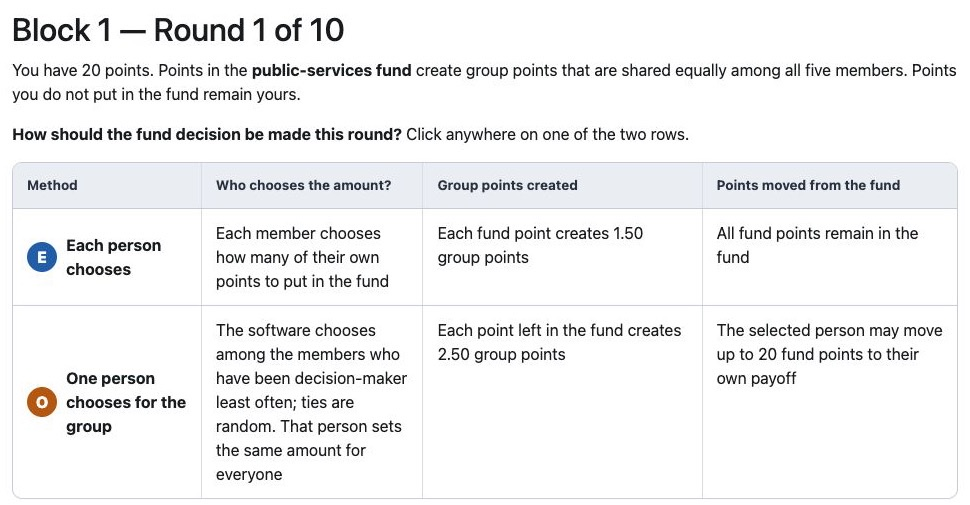
\includegraphics[width=0.97\linewidth]{interface_institution_choice.jpg}}}
\caption{Participant screen for choosing whether the leader's proposal requires approval.}
\label{fig:interface-choice}
\end{figure}

\paragraph{Leader proposal.} Under either rule, the leader proposes an equal allocation $t\in\{0,\ldots,20\}$ and a personal transfer $\rho\in\{0,\ldots,20\}$, with $\rho\leq5t$. Let $\pi$ denote a citizen's payoff in that round. Under \Aproc{}, the proposal takes effect directly, and a nonleader earns
\begin{equation}
\pi^{A}_{igbr}=20-t+\frac{2.50}{5}(5t-\rho),
\label{eq:automatic-nonleader}
\end{equation}
and the leader earns $\pi^{A,L}_{igbr}=\pi^{A}_{igbr}+\rho$.

\paragraph{Approval-constrained procedure (\Dproc).} The four nonleaders observe $(t,\rho)$ and vote privately; let $q_{igbr}=1$ denote approval. The proposal passes when at least three approve. If it passes, the payoffs above apply with $m_{gb}$ replacing 2.50. If it fails, each citizen chooses $c_{igbr}\in\{0,\ldots,20\}$ and earns
\begin{equation}
\pi^{D}_{igbr}=20-c_{igbr}+\frac{m_{gb}}{5}\sum_{j=1}^{5}c_{jgbr}.
\label{eq:approval-fallback}
\end{equation}
The rejected transfer is not implemented. Everyone then sees the proposal, approval total, implemented allocation, transfer, and own payoff.

\begin{plainlanguagebox}
Rejection restores the standard \textbf{public-goods dilemma}. If one citizen contributes 1 point and four contribute 0, the contributor earns $19+\frac{1.50}{5}=19.30$ during the crisis, while each free-rider earns $20.30$. Under recovery, these payoffs become $19.50$ and $20.50$. Contributing helps the group but costs the contributor; direct implementation avoids that risk, while approval lets citizens block an unwanted proposal.
\end{plainlanguagebox}

\begin{figure}[H]
\centering
\begin{minipage}[t]{0.49\textwidth}
\centering
\textbf{(a) Leader proposal}\par\smallskip
{\setlength{\fboxsep}{0pt}\setlength{\fboxrule}{0.4pt}%
\fbox{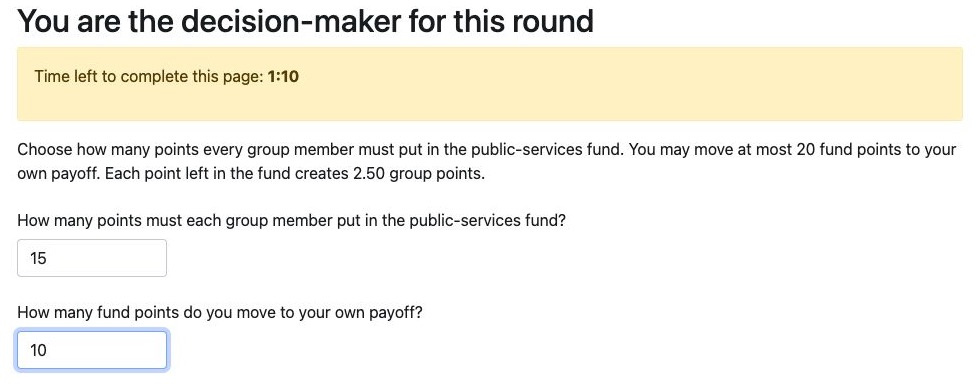
\includegraphics[width=0.97\linewidth]{interface_leader_allocation.jpg}}}
\end{minipage}\hfill
\begin{minipage}[t]{0.49\textwidth}
\centering
\textbf{(b) Citizen approval}\par\smallskip
{\setlength{\fboxsep}{0pt}\setlength{\fboxrule}{0.4pt}%
\fbox{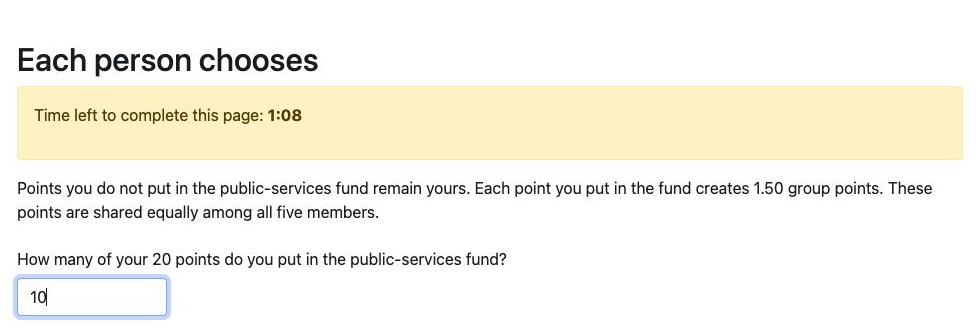
\includegraphics[width=0.97\linewidth]{interface_individual_allocation.jpg}}}
\end{minipage}

\vspace{0.8em}
\textbf{(c) Proposal, approval, and payoff feedback}\par\smallskip
{\setlength{\fboxsep}{0pt}\setlength{\fboxrule}{0.4pt}%
\fbox{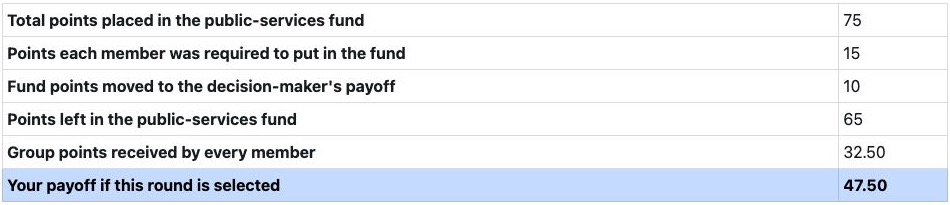
\includegraphics[width=0.91\linewidth]{interface_round_result.jpg}}}
\caption{Proposal, approval, and round feedback. Entered amounts are illustrative.}
\label{fig:interface-actions}
\end{figure}

\paragraph{How incentives map onto reversal.} During Block 1, \Aproc{} combines a 2.50 rate with guaranteed implementation; \Dproc{} uses 1.50 and may return to voluntary contributions after rejection. Recovery jointly reports improved public-service conditions and raises \Dproc{} to 2.50, while persistence retains the crisis and rate gap. The proposal set, approval rule, rejection procedure, and \Aproc{} rule remain unchanged. The recovery--persistence contrast therefore estimates the total effect of this structural package.

\paragraph{From institutional choice to (un)democratic reversal.} A citizen who moves from \Aproc{} to \Dproc{} first votes to let an unknown leader's proposal take effect without approval and later votes to restore that approval. The public-good incentives make this act consequential: \Aproc{} still guarantees that the leader's equal allocation takes effect after recovery, while \Dproc{} may produce rejection and free riding. A higher switching rate under recovery shows that structural change can cause citizens to withdraw support for a weakly constrained decision rule. Importantly: \emph{reversal is observed as a vote to restore a decision right, not as a declaration of democratic sentiment.}

\begin{payoffbox}
Suppose the leader proposes $t=10$ and $\rho=0$, and the proposal is approved under \Dproc{}. Holding that decision fixed gives:

\begin{center}
\renewcommand{\arraystretch}{1.15}
\begin{tabular}{lcc}
\toprule
& Approval required (\Dproc) & Direct implementation (\Aproc) \\
\midrule
Crisis or persistence & 25 points each & 35 points each \\
Recovery & 35 points each & 35 points each \\
\bottomrule
\end{tabular}
\end{center}

Recovery makes an approved \Dproc{} proposal equally productive; it does not make it pay more. \Aproc{} still guarantees implementation. {\bf The question is: \emph{when approval becomes equally productive, do citizens vote to restore it?}}
\end{payoffbox}

Participants report expected payoffs and transfers before the final Block-1 ballot and the first and final Block-2 ballots. Expected payoffs assess whether they understood the rules' relative performance; expected transfers trace beliefs about how leaders will use their discretion.


\begin{plainlanguagebox}
Five citizens cast private institutional ballots ($V_{i,b,r}$), after which the software selects a leader. That leader proposes $(t,\rho)$. Under \Dproc{}, three of four nonleaders must approve; rejection activates individual contributions $(c_{igbr})$. Under \Aproc{}, the proposal takes effect directly. Everyone sees the result and payoff before rematching within pool $g$.
\end{plainlanguagebox}

\subsection{Block 1: crisis and leader authorization}

After consent, participants practice proposing, approving, rejecting, and making individual allocations after rejection, then answer five comprehension questions. The interface never calls either method democratic or undemocratic.

Block 1 begins with the public-service crisis described above. Each fund point produces 1.50 under \Dproc{} and 2.50 under \Aproc{}. The leader may propose the same allocation and transfer under either rule; what differs is whether the other citizens can reject it.

Each paid round repeats the same sequence: institutional ballot, leader proposal, approval or direct implementation, any individual allocation following rejection, feedback, and rematching. Expectations are elicited before the final ballot, and one Block-1 round is selected for payment.

\subsection{Block 2: structural change and reversal}

After Block 1, pools are assigned to \emph{recovery} or \emph{persistence}. Recovery jointly reports that the budget passed, waiting times are falling, and planning resumed, and raises the \Dproc{} multiplier from 1.50 to 2.50. Persistence retains the crisis and 1.50 rate. The \Aproc{} rate, leader selection, proposal set, approval threshold, and rejection procedure remain unchanged. Together, the updated description and rate form the structural-recovery treatment.

The first Block-2 ballot measures immediate support for restoring approval; the final ballot measures sustained reversal and is primary. Expectations are elicited before both ballots, and questions about democratic constraints appear only after paid decisions. One Block-2 round is selected for payment.


\section{Outcomes, Process Measures, and Estimands}

Let \(\ind{\cdot}\) equal 1 when the condition inside braces is true and 0 otherwise. The final Block-1 ballot defines endorsement of automatic implementation as
\begin{equation}
A_{i1}=\ind{V_{i,1,10}=\Aproc}.
\end{equation}
For the theoretically relevant subgroup with $A_{i1}=1$, reversal is
\begin{equation}
R_i=\ind{V_{i,2,10}=\Dproc}.
\end{equation}
{\bf The primary estimand is the average treatment effect of structural recovery among Block-1 supporters of automatic implementation}:
\begin{equation}
\tau_R=\mathbb{E}[R_i(1)-R_i(0)\mid A_{i1}=1],
\end{equation}
where \(R_i(1)\) and \(R_i(0)\) are participant \(i\)'s potential outcomes under recovery and persistence. Recovery includes both improved public-service conditions and the 2.50 \Dproc{} rate; \(\tau_R\) is the total effect of that package. Because $A_{i1}$ is measured before assignment, subgroup membership is fixed before treatment. The primary test repeatedly reassigns recovery according to the prespecified pool-level procedure to evaluate how unusual the observed contrast is. Because \(\tau_R\) describes the average eligible citizen, the primary estimate weights eligible participants equally; a secondary analysis gives each pool equal weight. Regression estimates cluster uncertainty by pool and include a prespecified indicator for fifteen-person pools.

Immediate reversal is
\begin{equation}
R_i^{I}=\ind{V_{i,2,1}=\Dproc}\quad\text{for }A_{i1}=1.
\end{equation}
The same comparison applied to \(R_i^{I}\) estimates immediate support for restoration. The final-round outcome \(R_i\) remains primary because it records whether that choice persists.

\begin{plainlanguagebox}
The primary estimand ($\tau_R$) asks: among citizens who voted for direct implementation in Block 1's final round ($V_{i,1,10}=\Aproc$; $A_{i1}=1$), how much more often does recovery ($T_g=1$), rather than persistence ($T_g=0$), lead them to vote for group approval in Block 2's final round ($V_{i,2,10}=\Dproc$; $R_i=1$)? Only one potential outcome is observed per citizen, so random assignment identifies the difference. Assignment and inference operate at pool level.
\end{plainlanguagebox}

For each leader $i$, $t_{igbr}$ is the proposed allocation and $\rho_{igbr}$ the proposed transfer. A transfer proposal is $M_{igbr}=\ind{\rho_{igbr}>0}$, with intensity $\rho_{igbr}/(5t_{igbr})$ when $t_{igbr}>0$. Thus, $t=10$ and $\rho=5$ proposes moving 10\% of the 50 collected points. Approval ballots $q_{igbr}$, proposal passage, contributions after rejection, and subsequent institutional ballots provide descriptive process evidence. Because groups choose their rule, these measures do not identify separate causal effects of recovery.

Immediate reversal \(R_i^{I}\) records the first response to the structural package, before Block-2 interaction (see \autoref{fig:decision-timeline}). The primary outcome \(R_i\) records Round 10 after nine completed rounds. Secondary outcomes include late-round automatic-implementation support and realized group-level restoration.

Expected payoffs assess whether participants understood how recovery changed the rules' relative performance, while expected transfers trace beliefs about leader discretion. The final questionnaire checks perceived Block-1 crisis severity and Block-2 change, then records views on approval, equal allocation, and transfers. These measures assess the manipulation and aid interpretation; they do not by themselves identify why the treatment changed behavior.


\begin{figure}[H]
\centering
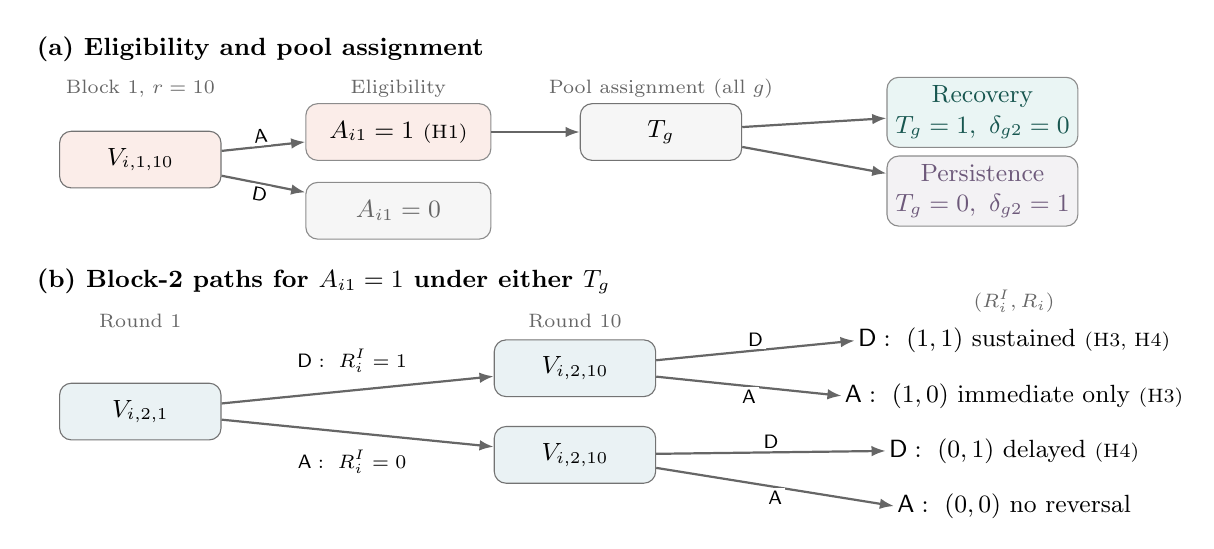
\begin{tikzpicture}[
  x=1.15cm,y=1cm,
  choice/.style={draw=black!55,rounded corners=1.5mm,fill=white,
                 align=center,minimum width=2.05cm,minimum height=0.72cm,
                 inner sep=3pt,font=\small},
  state/.style={draw=black!45,rounded corners=1.5mm,align=center,
                minimum width=2.35cm,minimum height=0.72cm,
                inner sep=3pt,font=\small},
  leaf/.style={align=left,font=\small,inner sep=1pt},
  flow/.style={-{Latex[length=1.8mm]},thick,draw=black!60},
  edge/.style={font=\scriptsize,fill=white,inner sep=1pt}
]
% Eligibility and pool-level assignment
\node[font=\small\bfseries,anchor=west] at (0,5.75)
  {(a) Eligibility and pool assignment};
\node[font=\scriptsize,text=black!60] at (1.25,5.25) {Block 1, $r=10$};
\node[font=\scriptsize,text=black!60] at (4.10,5.25) {Eligibility};
\node[font=\scriptsize,text=black!60] at (7.00,5.25) {Pool assignment (all $g$)};
\node[font=\scriptsize,text=black!60] at (10.55,5.25) {Block-2 condition};

\node[choice,fill=LightOrange] (b1vote) at (1.25,4.35) {$V_{i,1,10}$};
\node[state,fill=LightOrange] (eligible) at (4.10,4.70) {$A_{i1}=1$ {\scriptsize(H1)}};
\node[state,fill=gray!7,text=black!60] (outside) at (4.10,3.70) {$A_{i1}=0$};
\node[choice,fill=gray!7] (assign) at (7.00,4.70) {$T_g$};
\node[state,fill=RecoveryGreen!10,text=RecoveryGreen!55!black] (recovery) at (10.55,4.95)
  {Recovery\\$T_g=1,\ \delta_{g2}=0$};
\node[state,fill=PersistPurple!8,text=PersistPurple] (persistence) at (10.55,3.95)
  {Persistence\\$T_g=0,\ \delta_{g2}=1$};

\draw[flow] (b1vote) -- node[edge,above,sloped,pos=0.48] {$\Aproc$} (eligible);
\draw[flow] (b1vote) -- node[edge,below,sloped,pos=0.48] {$\Dproc$} (outside);
\draw[flow] (eligible) -- (assign);
\draw[flow] (assign) -- (recovery);
\draw[flow] (assign) -- (persistence);

% Block-2 paths within either assigned condition
\node[font=\small\bfseries,anchor=west] at (0,2.80)
  {(b) Block-2 paths for $A_{i1}=1$ under either $T_g$};
\node[font=\scriptsize,text=black!60] at (1.25,2.30) {Round 1};
\node[font=\scriptsize,text=black!60] at (6.05,2.30) {Round 10};
\node[font=\scriptsize,text=black!60] at (10.90,2.55) {$(R_i^{I},R_i)$};

\node[choice,fill=LightBlue] (b2first) at (1.25,1.15) {$V_{i,2,1}$};
\node[choice,fill=LightBlue] (finalupper) at (6.05,1.70) {$V_{i,2,10}$};
\node[choice,fill=LightBlue] (finallower) at (6.05,0.60) {$V_{i,2,10}$};

\node[leaf] (dd) at (10.90,2.05) {$\Dproc:\ (1,1)$ sustained {\scriptsize(H3, H4)}};
\node[leaf] (da) at (10.90,1.35) {$\Aproc:\ (1,0)$ immediate only {\scriptsize(H3)}};
\node[leaf] (ad) at (10.90,0.65) {$\Dproc:\ (0,1)$ delayed {\scriptsize(H4)}};
\node[leaf] (aa) at (10.90,-0.05) {$\Aproc:\ (0,0)$ no reversal};

\draw[flow] (b2first) -- node[edge,above=4pt,pos=0.48,inner sep=2pt] {$\Dproc:\ R_i^{I}=1$} (finalupper);
\draw[flow] (b2first) -- node[edge,below=4pt,pos=0.48,inner sep=2pt] {$\Aproc:\ R_i^{I}=0$} (finallower);
\draw[flow] (finalupper) -- node[edge,above] {$\Dproc$} (dd.west);
\draw[flow] (finalupper) -- node[edge,below] {$\Aproc$} (da.west);
\draw[flow] (finallower) -- node[edge,above] {$\Dproc$} (ad.west);
\draw[flow] (finallower) -- node[edge,below] {$\Aproc$} (aa.west);
\end{tikzpicture}
\caption{Decision tree for assignment and reversal. Each pool is assigned one value of $T_g$; the primary analysis follows participants with $A_{i1}=1$.}
\label{fig:decision-timeline}
\begin{minipage}{0.96\textwidth}
\footnotesize\emph{Notes:} The displayed ballots are $V_{i,1,10}$ (final Block 1), $V_{i,2,1}$ (first Block 2), and $V_{i,2,10}$ (final Block 2). The ordered pair $(R_i^{I},R_i)$ records the two Block-2 outcomes, with $1=\Dproc$ and $0=\Aproc$. Thus, $(1,1)$ is sustained reversal; $(1,0)$ immediate only; $(0,1)$ delayed; and $(0,0)$ no reversal. Parentheses identify the corresponding hypotheses; H2 concerns transfers and is not shown.
\end{minipage}
\end{figure}

\section{Randomization, Sample, and Power}

The planned sample comprises 300 completed participants in 28--30 matching pools. Ten-person pools are the default; no more than four fifteen-person pools are used, preserving at least 28 independent treatment assignments. Treatment is assigned only after everyone finishes Block 1. Within each session, pools are ordered by their final-round Block-1 \Aproc{} vote share and paired. One pool in each pair receives recovery and the other persistence, at random; an unmatched pool is assigned by a fair draw. Pairing improves balance in the number eligible to reverse, which is measured before assignment. The maximum payment of EUR~15 implies a participant-compensation ceiling of EUR~4,500 for 300 completed participants.

Power depends on Block-1 endpoint support for \Aproc{}, the persistence-group reversal rate, the similarity of outcomes within pools, and the realised mix of pool sizes. With 300 participants, the design yields 28--30 independent treatment assignments---approximately 14--15 pools per condition---because a larger pool supplies more individual outcomes but still receives only one treatment draw. Repeated rounds improve measurement and reveal trajectories; they do not create additional independent assignments.

Pilot estimates will inform simulations spanning 28--30 pools and the observed number eligible to reverse. The primary randomization test reproduces the actual paired and unmatched assignments. Regression estimates cluster uncertainty by pool, adjust for the prespecified pool-size indicator, and use small-sample inference; an equal-pool-weight analysis checks whether results depend on larger pools contributing more participants. Each oTree session remains a separate interaction and randomization cohort.

Strategic decisions do not time out automatically. The software records response time and flags decisions exceeding 90 seconds, but never generates a ballot or allocation. The laboratory manager monitors the session and prompts delayed participants to complete the current decision so the group can advance.

\FloatBarrier

\section{Implementation Plan}

The study will be conducted at the University of Turku PCRC Decision Laboratory after ethical approval. Adult participants join TOKA under its general laboratory rules and privacy notice. At the laboratory, oTree provides project-specific information and records a short affirmative study consent before practice. The laboratory manager then fixes a consenting roster divisible by five, forms 10- and, when needed, 15-person matching pools, and releases any surplus arrivals under PCRC procedures before paid play. No participant enters or changes pools after paid play begins.

The protocol will be piloted before production. A technical pilot will test 10- and 15-person pools, mixed-pool sessions, both Block-2 conditions, wait pages, rematching, response-time flags, browser recovery, exports, and payment calculations. A behavioral pilot will assess comprehension, session length, choice distributions, fatigue, and expected earnings. The protocol, analysis plan, and data dictionary will then be frozen before confirmatory data collection.

Production sessions will last approximately 60 minutes. The laboratory manager will monitor synchronized progress and prompt delayed participants; the software will record delays but will never generate a ballot, proposal, approval decision, or allocation. A structured session log will record late arrivals, early departures, technical interruptions, staff interventions, and payment exceptions. The research team will review the log before applying preregistered data-quality rules.

\section{Recruitment, Participant Care, and Resources}

The PCRC laboratory will invite adults through its participant pool using a neutral description of a paid study of group decision making and public-service provision. Recruitment will not disclose the directional hypotheses. Participation is voluntary and will not affect employment, studies, or access to University services. The fixed participation payment is EUR~10; points earned in one randomly selected round from each block determine a performance bonus of up to EUR~5.

Foreseeable risks are minimal. Participants may experience mild discomfort with unequal allocations, the fictional crisis, or waiting for an interacting group. Instructions avoid moral or partisan labels, individual ballots remain private, and only group-level outcomes are shown to other participants. The debrief explains the research interpretation only after paid decisions and emphasizes that no individual choice is treated as evidence of corruption, authoritarianism, or opposition to democracy.

Participant compensation is EUR~10--15, with a ceiling of EUR~4,500 for 300 completed participants. PCRC laboratory charges and any separate arrangements for timely arrivals who cannot enter a valid roster follow the institutional agreement. Secure data services and routine dissemination costs follow available project funds. The experiment uses the open-source oTree platform and requires no proprietary experimental-software licence.

\section{Data Governance, Schedule, and Outputs}

The experimental interface uses participant codes rather than names. The production oTree study and coded research data are hosted on University of Turku IT servers in Finland. PCRC keeps identifying recruitment and payment information separate and gives researchers only coded data. It retains the temporary identity-to-code link until compensation is paid and then deletes it. Access to coded research data is limited to Janne Tukiainen, Hector Bahamonde, and authorised personnel. Reporting will use aggregate or de-identified data, while coded data may be retained for verification and compatible future research under the privacy notice.

\begin{table}[H]
\centering
\caption{Planned project schedule}
\begin{tabularx}{0.92\textwidth}{@{}L{0.24\textwidth}X@{}}
\toprule
Period & Main activities \\
\midrule
September 2026 & Ethical review, final programming and translation, technical and behavioral pilots, data-protection review, and preregistration. \\
1--31 October 2026 & PCRC recruitment and laboratory data collection, subject to pool availability. \\
November--December 2026 & Data verification, de-identification, reproducible cleaning, primary and secondary analyses, and robustness checks. \\
January--March 2027 & Manuscript preparation and preparation of de-identified replication materials. \\
After reporting & Retention, controlled archiving, or deletion in accordance with the approved data management plan and privacy notice. \\
\bottomrule
\end{tabularx}
\end{table}

The main outputs will be academic articles, presentations, and replication materials. Consistent with University open-science policy, code, documentation, and data that can be shared safely will be made as open as possible and as restricted as necessary. The primary conclusion will follow the estimand and decision rule stated above; related econometric and randomization-based methods may be used to assess precision and robustness without changing the randomized comparison.

\printbibliography

\end{document}
